% Options for packages loaded elsewhere
\PassOptionsToPackage{unicode}{hyperref}
\PassOptionsToPackage{hyphens}{url}
\PassOptionsToPackage{dvipsnames,svgnames,x11names}{xcolor}
%
\documentclass[
  a4paper,
]{scrreport}

\usepackage{amsmath,amssymb}
\usepackage{lmodern}
\usepackage{iftex}
\ifPDFTeX
  \usepackage[T1]{fontenc}
  \usepackage[utf8]{inputenc}
  \usepackage{textcomp} % provide euro and other symbols
\else % if luatex or xetex
  \usepackage{unicode-math}
  \defaultfontfeatures{Scale=MatchLowercase}
  \defaultfontfeatures[\rmfamily]{Ligatures=TeX,Scale=1}
\fi
% Use upquote if available, for straight quotes in verbatim environments
\IfFileExists{upquote.sty}{\usepackage{upquote}}{}
\IfFileExists{microtype.sty}{% use microtype if available
  \usepackage[]{microtype}
  \UseMicrotypeSet[protrusion]{basicmath} % disable protrusion for tt fonts
}{}
\makeatletter
\@ifundefined{KOMAClassName}{% if non-KOMA class
  \IfFileExists{parskip.sty}{%
    \usepackage{parskip}
  }{% else
    \setlength{\parindent}{0pt}
    \setlength{\parskip}{6pt plus 2pt minus 1pt}}
}{% if KOMA class
  \KOMAoptions{parskip=half}}
\makeatother
\usepackage{xcolor}
\setlength{\emergencystretch}{3em} % prevent overfull lines
\setcounter{secnumdepth}{5}
% Make \paragraph and \subparagraph free-standing
\ifx\paragraph\undefined\else
  \let\oldparagraph\paragraph
  \renewcommand{\paragraph}[1]{\oldparagraph{#1}\mbox{}}
\fi
\ifx\subparagraph\undefined\else
  \let\oldsubparagraph\subparagraph
  \renewcommand{\subparagraph}[1]{\oldsubparagraph{#1}\mbox{}}
\fi


\providecommand{\tightlist}{%
  \setlength{\itemsep}{0pt}\setlength{\parskip}{0pt}}\usepackage{longtable,booktabs,array}
\usepackage{calc} % for calculating minipage widths
% Correct order of tables after \paragraph or \subparagraph
\usepackage{etoolbox}
\makeatletter
\patchcmd\longtable{\par}{\if@noskipsec\mbox{}\fi\par}{}{}
\makeatother
% Allow footnotes in longtable head/foot
\IfFileExists{footnotehyper.sty}{\usepackage{footnotehyper}}{\usepackage{footnote}}
\makesavenoteenv{longtable}
\usepackage{graphicx}
\makeatletter
\def\maxwidth{\ifdim\Gin@nat@width>\linewidth\linewidth\else\Gin@nat@width\fi}
\def\maxheight{\ifdim\Gin@nat@height>\textheight\textheight\else\Gin@nat@height\fi}
\makeatother
% Scale images if necessary, so that they will not overflow the page
% margins by default, and it is still possible to overwrite the defaults
% using explicit options in \includegraphics[width, height, ...]{}
\setkeys{Gin}{width=\maxwidth,height=\maxheight,keepaspectratio}
% Set default figure placement to htbp
\makeatletter
\def\fps@figure{htbp}
\makeatother

\usepackage{venndiagram}
\newcommand{\NN}{\mathbb{N}}
\newcommand{\ZZ}{\mathbb{Z}}
\newcommand{\QQ}{\mathbb{Q}}
\newcommand{\RR}{\mathbb{R}}
\newcommand{\CC}{\mathbb{C}}
\DeclareMathOperator{\operatorname{Int}}{Int}
\DeclareMathOperator{\operatorname{Ext}}{Ext}
\DeclareMathOperator{\operatorname{Fr}}{Fr}
\DeclareMathOperator{\Adh}{Adh}
\DeclareMathOperator{\Ac}{Ac}
\DeclareMathOperator{\sen}{sen}
\makeatletter
\makeatother
\makeatletter
\@ifpackageloaded{bookmark}{}{\usepackage{bookmark}}
\makeatother
\makeatletter
\@ifpackageloaded{caption}{}{\usepackage{caption}}
\AtBeginDocument{%
\ifdefined\contentsname
  \renewcommand*\contentsname{Tabla de contenidos}
\else
  \newcommand\contentsname{Tabla de contenidos}
\fi
\ifdefined\listfigurename
  \renewcommand*\listfigurename{Listado de Figuras}
\else
  \newcommand\listfigurename{Listado de Figuras}
\fi
\ifdefined\listtablename
  \renewcommand*\listtablename{Listado de Tablas}
\else
  \newcommand\listtablename{Listado de Tablas}
\fi
\ifdefined\figurename
  \renewcommand*\figurename{Figura}
\else
  \newcommand\figurename{Figura}
\fi
\ifdefined\tablename
  \renewcommand*\tablename{Tabla}
\else
  \newcommand\tablename{Tabla}
\fi
}
\@ifpackageloaded{float}{}{\usepackage{float}}
\floatstyle{ruled}
\@ifundefined{c@chapter}{\newfloat{codelisting}{h}{lop}}{\newfloat{codelisting}{h}{lop}[chapter]}
\floatname{codelisting}{Listado}
\newcommand*\listoflistings{\listof{codelisting}{Listado de Listados}}
\makeatother
\makeatletter
\@ifpackageloaded{caption}{}{\usepackage{caption}}
\@ifpackageloaded{subcaption}{}{\usepackage{subcaption}}
\makeatother
\makeatletter
\@ifpackageloaded{tcolorbox}{}{\usepackage[many]{tcolorbox}}
\makeatother
\makeatletter
\@ifundefined{shadecolor}{\definecolor{shadecolor}{rgb}{.97, .97, .97}}
\makeatother
\makeatletter
\makeatother
\ifLuaTeX
\usepackage[bidi=basic]{babel}
\else
\usepackage[bidi=default]{babel}
\fi
\babelprovide[main,import]{spanish}
% get rid of language-specific shorthands (see #6817):
\let\LanguageShortHands\languageshorthands
\def\languageshorthands#1{}
\ifLuaTeX
  \usepackage{selnolig}  % disable illegal ligatures
\fi
\IfFileExists{bookmark.sty}{\usepackage{bookmark}}{\usepackage{hyperref}}
\IfFileExists{xurl.sty}{\usepackage{xurl}}{} % add URL line breaks if available
\urlstyle{same} % disable monospaced font for URLs
\hypersetup{
  pdftitle={Prácticas de Estadística con R},
  pdfauthor={Alfredo Sánchez Alberca},
  pdflang={es},
  colorlinks=true,
  linkcolor={blue},
  filecolor={Maroon},
  citecolor={Blue},
  urlcolor={Blue},
  pdfcreator={LaTeX via pandoc}}

\title{Prácticas de Estadística con R}
\author{Alfredo Sánchez Alberca}
\date{6/1/22}

\begin{document}
\begin{titlepage}

%\AddToShipoutPicture*{\put(0,0){\includegraphics[scale=0.8]{img/background2}}} % Imagen de fondo, requiere el paquete eso-pic.
\begin{center}
\vspace*{5cm}

\Huge
{\textbf{\textsf{Prácticas de Estadística con R}}}

\vspace{0.5cm}
\LARGE
{\textbf{\textsf{}}}

\vspace{1.5cm}

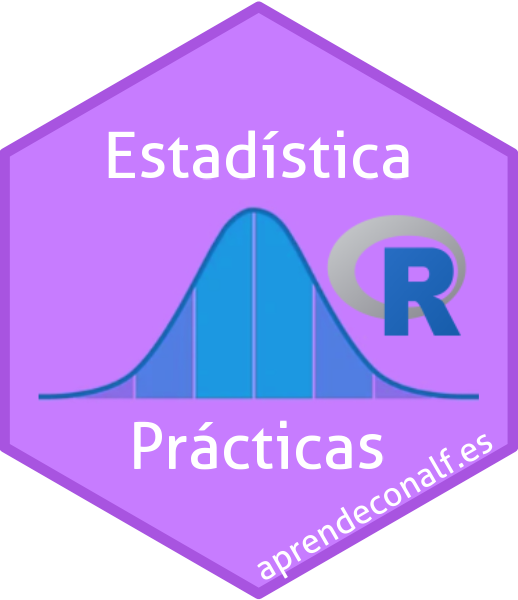
\includegraphics[width=0.4\textwidth]{img/logos/sticker-estadistica-r.png}
\end{center}

\vfill

\begin{flushleft}
\begin{tabular}{ll}

\includegraphics[width=0.1\textwidth]{img/logos/aprendeconalf.png} & \parbox[b]{5cm}{\Large\textsf{Alfredo
Sánchez
Alberca}\\ \textsf{asalber@ceu.es} \\ \textsf{https://aprendeconalf.es}}
\end{tabular}
\end{flushleft}
\end{titlepage}\ifdefined\Shaded\renewenvironment{Shaded}{\begin{tcolorbox}[boxrule=0pt, frame hidden, interior hidden, borderline west={3pt}{0pt}{shadecolor}, breakable, enhanced, sharp corners]}{\end{tcolorbox}}\fi

\renewcommand*\contentsname{Tabla de contenidos}
{
\hypersetup{linkcolor=}
\setcounter{tocdepth}{2}
\tableofcontents
}
\bookmarksetup{startatroot}

\hypertarget{prefacio}{%
\chapter*{Prefacio}\label{prefacio}}
\addcontentsline{toc}{chapter}{Prefacio}

\markboth{Prefacio}{Prefacio}

¡Bienvenido a Prácticas de Estadística con R!

Este libro presenta una recopilación de prácticas de Estadística
Descriptiva e Inferencial con el lenguaje de programación
\href{https://www.r-project.org/}{R}, con problemas aplicados a las
Ciencias y las Ingenierías.

No es un libro para aprender a programar con R, ya que solo enseña el
uso del lenguaje y de algunos de sus paquetes para resolver problemas de
Estadística. Para quienes estén interesados en aprender a programar en
este lenguaje, os recomiendo leer este
\href{https://aprendeconalf.es/manual-r/}{manual de R}.

\hypertarget{licencia}{%
\section*{Licencia}\label{licencia}}
\addcontentsline{toc}{section}{Licencia}

\markright{Licencia}

Esta obra está bajo una licencia Reconocimiento -- No comercial --
Compartir bajo la misma licencia 3.0 España de Creative Commons. Para
ver una copia de esta licencia, visite
\url{https://creativecommons.org/licenses/by-nc-sa/3.0/es/}.

Con esta licencia eres libre de:

\begin{itemize}
\tightlist
\item
  Copiar, distribuir y mostrar este trabajo.
\item
  Realizar modificaciones de este trabajo.
\end{itemize}

Bajo las siguientes condiciones:

\begin{itemize}
\item
  \textbf{Reconocimiento}. Debe reconocer los créditos de la obra de la
  manera especificada por el autor o el licenciador (pero no de una
  manera que sugiera que tiene su apoyo o apoyan el uso que hace de su
  obra).
\item
  \textbf{No comercial}. No puede utilizar esta obra para fines
  comerciales.
\item
  \textbf{Compartir bajo la misma licencia}. Si altera o transforma esta
  obra, o genera una obra derivada, sólo puede distribuir la obra
  generada bajo una licencia idéntica a ésta.
\end{itemize}

Al reutilizar o distribuir la obra, tiene que dejar bien claro los
términos de la licencia de esta obra.

Estas condiciones pueden no aplicarse si se obtiene el permiso del
titular de los derechos de autor.

Nada en esta licencia menoscaba o restringe los derechos morales del
autor.

\bookmarksetup{startatroot}

\hypertarget{introducciuxf3n-a-r}{%
\chapter{Introducción a R}\label{introducciuxf3n-a-r}}

La gran potencia de cómputo alcanzada por los ordenadores ha convertido
a los mismos en poderosas herramientas al servicio de todas aquellas
disciplinas que, como la Estadística, requieren manejar un gran volumen
de datos. Actualmente, prácticamente nadie se plantea hacer un estudio
estadístico serio sin la ayuda de un buen programa de análisis de datos.

\emph{R} es un potente lenguaje de programación que incluye multitud de
funciones para la representación y el análisis de datos. Fue
desarrollado por Robert Gentleman y Ross Ihaka en la Universidad de
Auckland en Nueva Zelanda, aunque actualmente es mantenido por una
enorme comunidad científica en todo el mundo.

\begin{figure}

{\centering 
\includegraphics[width=0.25\textwidth,height=\textheight]{./img/logos/Rlogo.png}

}

\caption{Logotipo de R}

\end{figure}

Las ventajas de R frente a otros programas habituales de análisis de
datos, como pueden ser SPSS, SAS o Matlab, son múltiples:

\begin{itemize}
\tightlist
\item
  Es software libre y por tanto gratuito. Puede descargarse desde la web
  \url{http://www.r-project.org/}.
\item
  Es multiplataforma. Existen versiones para Windows, Macintosh, Linux y
  otras plataformas.
\item
  Está avalado y en constante desarrollo por una amplia comunidad
  científica distribuida por todo el mundo que lo utiliza como estándar
  para el análisis de datos.
\item
  Cuenta con multitud de paquetes para todo tipo de análisis
  estadísticos y representaciones gráficas, desde los más habituales,
  hasta los más novedosos y sofisticados que no incluyen otros
  programas. Los paquetes están organizados y documentados en un
  \href{https://cran.r-project.org/}{repositorio CRAN} (Comprehensive R
  Archive Network) desde donde pueden descargarse libremente.
\item
  Es programable, lo que permite que el usuario pueda crear fácilmente
  sus propias funciones o paquetes para análisis de datos específicos.
  Existen multitud de libros, manuales y tutoriales libres que permiten
  su aprendizaje e ilustran el análisis estadístico de datos en
  distintas disciplinas científicas como las Matemáticas, la Física, la
  Biología, la Psicología, la Medicina, etc.
\end{itemize}

\hypertarget{instalaciuxf3n-de-r}{%
\section{Instalación de R}\label{instalaciuxf3n-de-r}}

R puede descargarse desde el \href{https://www.r-project.org/}{sitio web
oficial de R} o desde el repositorio principal de paquetes de R
\href{https://cran.r-project.org/}{CRAN}. Basta con descargar el archivo
de instalación correspondiente al sistema operativo de nuestro ordenador
y realizar la instalación como cualquier otro programa.

El intérprete de R se arranca desde la terminal, aunque en Windows
incorpora su propia aplicación, pero es muy básica. En general, para
trabajos serios, conviene utilizar un entorno de desarrollo para R.

\hypertarget{entornos-de-desarrollo}{%
\section{Entornos de desarrollo}\label{entornos-de-desarrollo}}

Por defecto el entorno de trabajo de R es en línea de comandos, lo que
significa que los cálculos y los análisis se realizan mediante comandos
o instrucciones que el usuario teclea en una ventana de texto. No
obstante, existen distintas interfaces gráficas de usuario que facilitan
su uso, sobre todo para usuarios noveles. Algunas de ellas, como las que
se enumeran a continuación, son completos entornos de desarrollo que
facilitan la gestión de cualquier proyecto:

\begin{itemize}
\item
  \href{https://www.rstudio.com/}{RStudio}. Probablemente el entorno de
  desarrollo más extendido para programar con R ya que incorpora
  multitud de utilidades para facilitar la programación con R.
\item
  \href{https://rkward.kde.org}{RKWard}. Es otra otro de los entornos de
  desarrollo más completos que además incluye a posibilidad de añadir
  nuevos menús y cuadros de diálogo personalizados.
\item
  \href{https://code.visualstudio.com/}{Visual Studio Code}. Es un
  entorno de desarrollo de propósito general ampliamente extendido.
  Aunque no es un entorno de desarrollo específico para R, incluye una
  extensión con utilidades que facilitan mucho el desarrollo con R.
\end{itemize}

\bookmarksetup{startatroot}

\hypertarget{estaduxedstica-descriptiva}{%
\chapter{Estadística Descriptiva}\label{estaduxedstica-descriptiva}}

Prueba.



\end{document}
